\section*{Теория}
\addcontentsline{toc}{section}{Теория}
Как уже сообщалось выше, моделируемая система представляет собой тело, подвешенное в поле силы тяжести на нерастяжимой нити. Отсюда его базовые характеристики --- масса $m$ и длина $l$. Другие начальные условия, определяющие движение маятника --- начальное отклонение от вертикали (оно же $x_0$) и начальная скорость ($v_0$). 
\subsection*{Простой математический маятник}
\addcontentsline{toc}{subsection}{Простой математический маятник}
Самая простая модель маятника --- это математический маятник. В этом случае единственной существенной силой будет сила тяжести. Мы так же пренебрегаем размерами тела. Движение такой модели не будет зависить от массы маятника, и это видно по формулам, приведенным ниже.
\begin{figure}[h!]
	\centering
	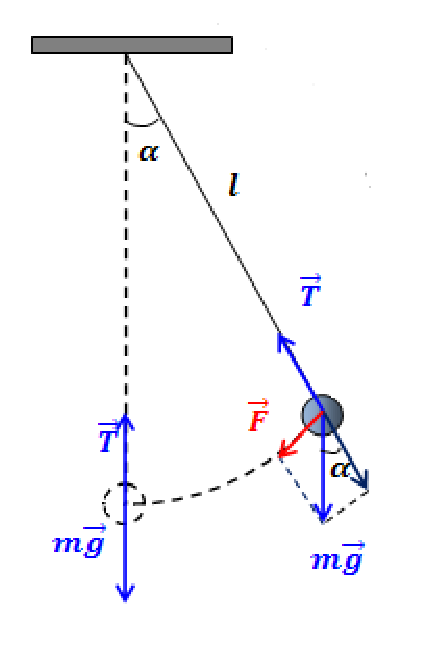
\includegraphics{mathp1}\\
	\caption{Силы, действующие на математический маятник }
\end{figure} \\ \\
Красным цветом на рисунке обозначена тангенциальная составляющая силы тяжести --- $\vec F_t$. Ее значение: $F_t = mg\sin\alpha$.\\
В соответсвии со вторым законом Ньютона: 
\begin{equation}
\vec a_t = \frac{\vec F_t} {m} 
\end{equation}
Получим $a_t = -g\sin\alpha$\\
Тангенциальное ускорение связано с углом таким образом:
\begin{equation}
\vec a_t = l\frac{d^2\alpha}{dt^2}
\end{equation}
Получим:
\begin{equation}
 l\frac{d^2\alpha}{dt^2} = -gsin\alpha
\end{equation}
Обозначим \begin{equation}\omega = \sqrt{\frac{g}{l}} \end{equation}
\begin{equation}
\frac{d^2\alpha}{dt^2} = -\omega^2sin\alpha
\end{equation}
Ограничимся случаем малых колебаний: $\sin\alpha \approx \alpha$ \\
Тогда:
\begin{equation}
\frac{d^2\alpha}{dt^2} = -\omega^2\alpha
\end{equation}
Решением этого уравнения будет:
\begin{equation}
\alpha(t) = A_\alpha\sin(\omega t + \alpha_0)
\end{equation}
$A$ и $\alpha_0$ задаются начальными условиями.\\
Координата $x_0$ связана с углом $\alpha$ следующим соотношением: $x_0=l\sin\alpha\approx l\alpha$
Тогда уравнение движения имеет вид:
\begin{equation}
x (t) = A_\alpha l\sin(\omega t + \alpha_0)
\end{equation}
или
\begin{equation}
x (t) = A\sin(\omega t + \alpha_0) 
\end{equation}
В описании маятника на C++ используются формулы (4) и (9). Из формулы (4) появляется новая характеристика --- циклическая частота. Еще одной характеристикой маятника является период --- время, за которое совершается одно колебание. Период связан с частотой следующим образом:
\begin{equation}
T = \frac{2\pi}{\omega}
\end{equation}
Найдем значения амплитуды $A$ и начального угла отклонения (или фазы) $\alpha_0$ из уравнений для $x$ и $x'$:
\begin{equation}
A = \sqrt{{x_0}^2 + {(\frac{v_0}{\omega})}^2}
\end{equation}
\begin{equation}
\alpha_0 = \arctan{\frac{x_0}{v_0}}
\end{equation}
Если $x_0 = v_0 = 0$, то $A = \alpha = 0$. \\
Как видим, движение математического маятника действительно не зависит от массы.\\
\subsection*{Маятник Фуко}
\addcontentsline{toc}{subsection}{Маятник Фуко}
Маятник Фуко --- это математический маятник, плоскость колебаний которого медленно поворачивается относительно земной поверхности в сторону, противоположную направлению вращения Земли. Это происходит из-за того, что на маятник действует сила Кориолиса.
\begin{figure}[h!]
	\begin{minipage}[h]{0.49\linewidth}
		\centering
		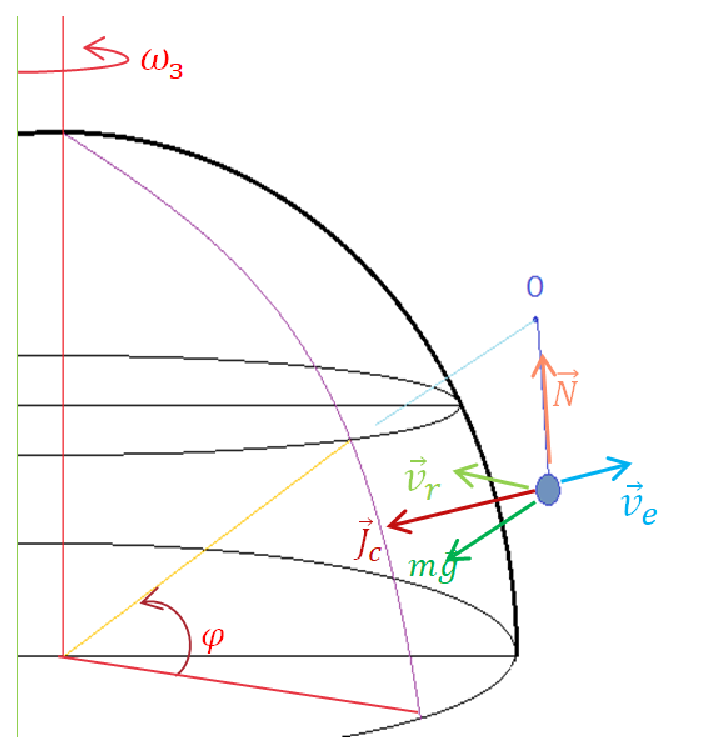
\includegraphics[width=0.5\linewidth]{fou1}\\
		\caption{Силы, действующие на маятник Фуко \label{fig:fou1}}
	\end{minipage}
	\begin{minipage}[h]{0.49\linewidth}
		\centering
		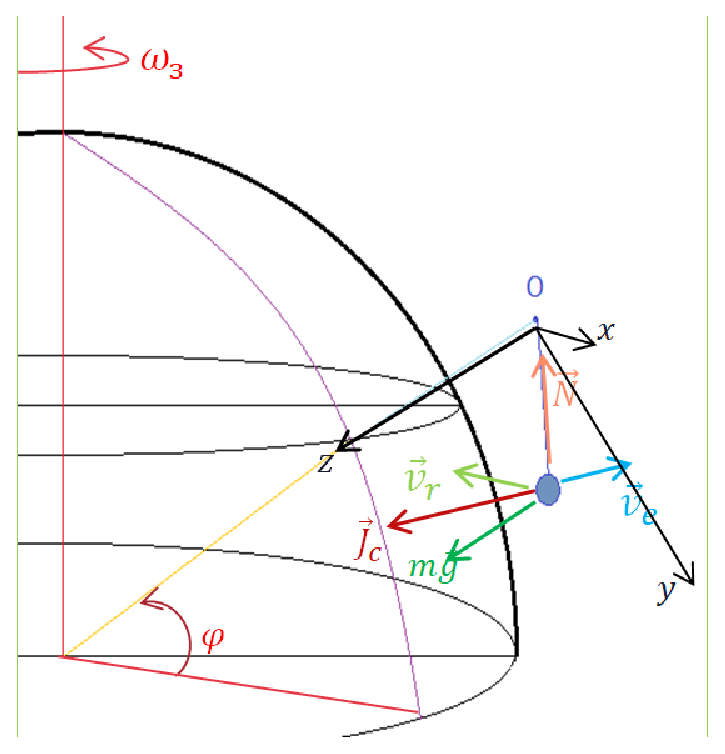
\includegraphics[width=0.5\linewidth]{fou2}\\
		\caption{Система координат $Oxyz$ \label{fig:fou2}}
	\end{minipage}
\end{figure} 
\clearpage
$J_c$ --- сила Кориолиса, $N$ --- сила натяжения нити, $\varphi$ --- географическая широта. $N_x = -\frac{nx}{l}$, $N_y = -\frac{ny}{l}$, $N_z = -\frac{nz}{l}$. 
Поместим начало координат в точку подвеса $O$. Ось $Oz$ направим вдоль отвесной линии (желтым), ось $Oy$ перпендикулярно $Oz$ в плоскости меридиана (по касательной к нему) и $Oy$ по касательной к плоскости параллели. $Ox \perp Oy \perp Oz$.\\
Так как нить нерастяжимая, то
\begin{equation}
x^2 + y^2 + z^2 = l^2
\end{equation}
Проекции сил, действующих на маятник Фуко:
\begin{equation}
m\ddot{x} = -\frac{nx}{l} + 2m\omega_{з} (\dot{z}\cos\varphi - \dot{y}\sin\varphi)
\end{equation}
\begin{equation}
m\ddot{y} = -\frac{ny}{l} + 2m\omega_{з}\dot{x}\sin\varphi
\end{equation}
\begin{equation}
m\ddot{z} = -\frac{nz}{l} - 2m\omega_{з}\dot{x}\cos\varphi - mg
\end{equation}
Как и в случае с математическим маятником рассмотрим только малые колебания маятника.
Тогда $x \ll l, y \ll l,  \dot{x} \ll \sqrt{gl},  \dot{y} \ll \sqrt{gl}$\\
$z = \sqrt{l^2 - x^2 - y^2} \approx 1 - \frac{x^2}{2l^2} - \frac{y^2}{2l^2} \approx l $ \\
Продифференциируем (13) по времени:
$\dot{z} = - \frac{x\dot{x}}{z} - \frac{y\dot{y}}{z} \approx   - \frac{x\dot{x}}{l} - \frac{y\dot{y}}{l} $  \\
Отсюда 
\begin{equation} \dot{z} \ll \dot{x} \dot{z} \ll \dot{y}  \end{equation}
Продифференциируем предыдущее выражени по времени:
\begin{equation} \frac{\ddot{z}}{g} = - \frac{\dot{x}\ddot{x}}{gl}  - \frac{\dot{y}\ddot{y}}{gl}  - \frac{\dot{x}^2}{gl}  - \frac{\dot{y}^2}{gl} \ll 1 \end{equation}
$\ddot{z} \ll g$
Так как угловая скорость Земли достаточно мала $\omega_{з} \ll \sqrt{g/l}  \Rightarrow  \omega_{з}\sqrt{gl} \ll g $ \\
Следовательно, $\omega_{з}x \ll  \omega_{з}\sqrt{gl} \ll  g $\\
Пренебрегая малыми слагаемыми получим для (16):
\begin{equation}
\frac{nz}{l} = mg
\end{equation}
$n \approx mg$\\
Тогда (14) и (15):
\begin{equation}
\ddot{x} = - \omega^{2}x - 2\omega_{*}\dot{y}
\end{equation}
\begin{equation}
\ddot{y} = - \omega^{2}y + 2\omega_{*}\dot{x}
\end{equation}
Где $\omega_{*} = \omega_{з}\sin\varphi$.\\
Умножим уравнение (20) на $-y$, (21) на $x$ и сложим:
\begin{equation}
x\ddot{y} - y\ddot{y} = 2\omega_{*}(x\dot{x} + y\dot{y})
\end{equation}
\begin{equation}
\frac{d(x\dot{y} - y\dot{x})}{dt}  = \omega_{*}\frac{d(x^2 + y^2)}{dt}
\end{equation}
Введем полярную систему координат: $x = \rho\cos\theta, y = \rho\sin\theta $\\
Тогда дифференциальное уравнение примет вид:
\begin{equation}
\frac{d\rho^2\dot{\theta}}{dt}  = \omega_{*}\frac{d\rho^2}{dt}
\end{equation}
Его интегрирование дает:
\begin{equation}
\rho^2\dot{\theta}  = \omega_{*}\rho^2 + С_1
\end{equation}
Отсюда при $t =0 \rho = 0   \theta = \omega_{*}t $\\
Найдем $\rho$:\\
Умножим (20) на $x$ и (21) на $y$. Сложим:
\begin{equation}
x\ddot{x} + y\ddot{y} = -\omega^{2}(x^2 + y^2) + 2\omega_{*}(\dot{x}y - \dot{y}x)
\end{equation}
Отсюда:
\begin{equation}
\ddot{\rho} + \omega_{1}^{2}\rho = 0
\end{equation}
Где $\omega_{1} = \omega^2 + \omega_{*}^2 \approx \omega^2$.\\
Получим уравнение движения  в полярных координатах:
\begin{equation}
\rho = \beta\sin(\omega_{1}t+ \gamma)
\end{equation}
Где $\beta$ и $\gamma$ находятся из начальных условий:
\begin{equation}
\gamma = \arctan\frac{\omega_{1}\cos\theta}{\frac{v_0}{x_0} + \omega_{*}\sin\theta}\\
\beta = \frac{x_0}{\sin\gamma}
\end{equation}
Если $x_0 = 0$, то $\gamma = 0, \beta = \frac{v_0}{\omega_{1}\cos\theta}$
\subsection*{Физический маятник}
\addcontentsline{toc}{subsection}{Физический маятник}
Физическим маятником называется твердое тело, закрепленное на неподвижной горизонтальной ocи (оси подвеса), не проходящей через центр тяжести, и совершающее колебания относительно этой оси под действием силы тяжести. В отличие от математического маятника массу такого тела нельзя считать точечной. В положение равновесия его возвращает та же тангенциальная составляющая силы тяжести --- $F_t = -mg\sin\alpha \approx -mg\alpha $. У физического маятника появляются новые значащие характеристики --- форма, ``радиус'', момент инерции и приведенная длина.\\
Дифференциальное уравнение колебаний физического маятника имеет вид:
\begin{equation}
\frac{d^2\alpha}{dt} + \frac{mgl}{J}\alpha = 0
\end{equation}
Где $J$ --- момент импульса.
\begin{figure}[h!]
	\centering
	\includegraphics[width = 0.7\linewidth]{phyp1}\\
	\caption{Формула для момента импульса}
\end{figure} \\ \\
Решение этого уравнения:
\begin{equation}
\alpha(t) = A_\alpha\sin(\omega t + \alpha_0)
\end{equation}
\begin{equation}
\omega = \sqrt {\frac{mgl}{g}}
\end{equation}
Найдем длину математического маятника, уравнение движения которого совпадает с (31). Такая длина называется \textbf{приведенная длина}:
\begin{equation}
L = \frac{J}{ml}
\end{equation}
\subsection*{Маятник с вязким трением}
\addcontentsline{toc}{subsection}{Маятник с вязким трением}
Силы трения, зависящие от значения скорости движущегося тела, у которых трение покоя отсутствует, называются силами вязкого трения. \\
$F_{тр} = -kv$, где $k$ --- динамическая вязкость. Например, вязкость воздуха --- 18,6 мкПа*с \\
Уравнение его движения:
\begin{equation}
\ddot{x} + 2c\dot{x} + \omega_{0}^{2}x = 0
\end{equation}
$ c = \frac{k}{2m} $\\
$ \omega_{0} = \sqrt{\frac{g}{l}} $ \\
Имеет три решения в зависимости от $c$.
\begin{enumerate}
\item		$
			c < \omega_{0}
		$
		\begin{equation}
			x (t) = Ae^{-ct}\sin(\omega t + \alpha_0) 
		\end{equation}
		\begin{equation}
			\omega = \sqrt{\omega_{0}^{2} - c^2}
		\end{equation}
		\begin{equation}
			A = \sqrt{x_{0}^{2} + ({\frac{v_0 + cx_0}{\omega}})^{2}}
		\end{equation}
		\begin{equation}
			\alpha = \arcsin{\frac{x_0}{A}}
		\end{equation}
\item       
		$c = \omega_{0}$
		\begin{equation}
			x = e^{-ct}(C_1 + C_{2}t)
		\end{equation}
		\begin{equation}
			C_1 = x_0
		\end{equation}
		\begin{equation}
			C_2 = v_0 + cx_0
		\end{equation}
\item
		$
			c > \omega_{0}
		$
		\begin{equation}
			x = C_{1}e^{-\gamma_{1}t} + C_{2}e^{-\gamma_{2}t}
		\end{equation}
		\begin{equation}
			\gamma_{1,2} = -c \pm \sqrt{c^2 - \omega_{0}^{2}}
		\end{equation}
		\begin{equation}
			C_{1} = \frac{v_0 - \gamma_{2}x0}{\gamma_1 - \gamma_2}
		\end{equation}
		\begin{equation}
			C_{2} = \frac{v_0 - \gamma_{2}x0}{\gamma_2 - \gamma_1}
		\end{equation}
\end{enumerate}
\begin{figure}[h!]
        \begin{minipage}[h]{0.32\linewidth}
	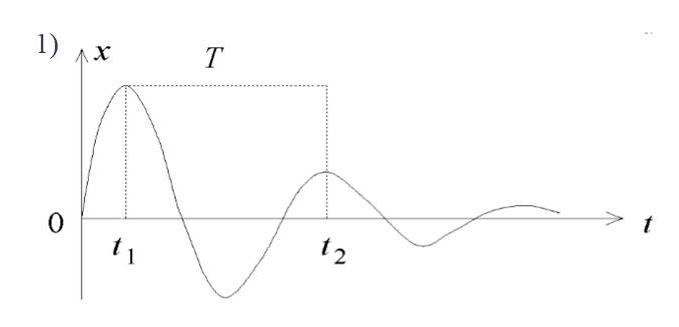
\includegraphics[width = 0.8\linewidth]{pwf1}\\
	\caption{Уравнение (35)}
	\end{minipage}
	\begin{minipage}[h]{0.32\linewidth}
	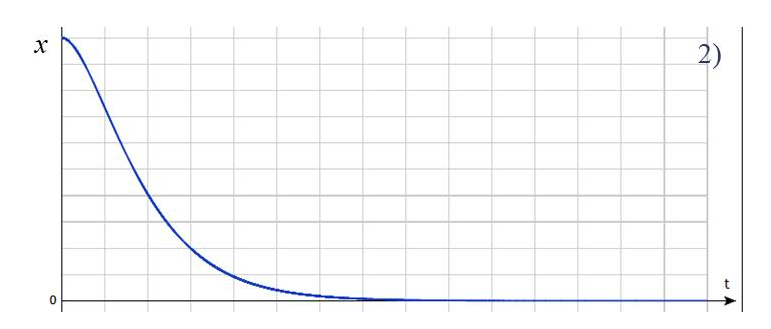
\includegraphics[width = 0.8\linewidth]{pwf2}\\
	\caption{Уравнение (39)}
	\end{minipage}
	\begin{minipage}[h]{0.32\linewidth}
	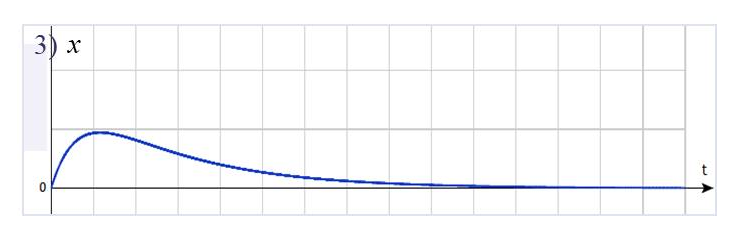
\includegraphics[width = 0.85\linewidth]{pwf3}\\
	\caption{Уравнение (42)}
	\end{minipage}
\end{figure} 
